\documentclass[a4paper,12pt]{article}
%\pagestyle{empty}
\usepackage{geometry}
 \geometry{
 a4paper,
 total={170mm,257mm},
 left=20mm,
 top=20mm,
 }
\usepackage{graphicx}
\usepackage{amssymb}
\usepackage{enumitem}
\usepackage{amsmath, amsthm, amssymb, listings, multirow, wrapfig}
\newcommand{\bigCI}{\mathrel{\text{\scalebox{1.07}{$\perp\mkern-10mu\perp$}}}}
\usepackage{amsmath,amsfonts,stmaryrd,amssymb} % Math packages
\usepackage{algorithm}
\usepackage{algorithmic}
\usepackage{enumerate} % Custom item numbers for enumerations
\usepackage{tikz}
\usepackage[colorlinks=true,citecolor=blue]{hyperref}%
\usetikzlibrary{arrows}
%\usepackage[ruled]{algorithm2e} % Algorithms

\usepackage[framemethod=tikz]{mdframed} % Allows defining custom boxed/framed environments

\usepackage{listings} % File listings, with syntax highlighting
\lstset{
	basicstyle=\ttfamily, % Typeset listings in monospace font
}

\usepackage{xepersian}

\usepackage{bbm}
\settextfont[Scale=1]{Nazli}
%\setlatintextfont{Serif}
\setdigitfont[Scale=1.2]{Yas}
\DefaultMathsDigits
\renewcommand{\labelitemi}{$\circ$}

\newtheorem{den}{{\large\bf تعریف}}[section]
\newtheorem{exa}{{\large\bf مثال}}[section]
\newtheorem{lem}{{\large\bf لم}}[section]
\newtheorem{pro}{{\large\bf گزاره}}[section]
\newtheorem{cor}{{\large\bf نتیجه}}[section]
\newtheorem{thm}{{\large\bf قضیه}}[section]
\newtheorem{rem}{{\large\bf تذکر}}[section]
\newtheorem{nnt}{{\large\bf توجه}}[section]

%\newenvironment{proof}{{\bf اثبات.} \rm }{\hfill{$\blacksquare$}}
\newcommand{\bt}{\begin{theorem}}
	\newcommand{\et}{\end{theorem}}
\newcommand{\bl}{\begin{lemma}}
	\newcommand{\el}{\end{lemma}}
\newcommand{\bc}{\begin{corollary}}
	\newcommand{\ec}{\end{corollary}}
\newcommand{\bp}{\begin{proof}}
	\newcommand{\ep}{\end{proof}}
\newcommand{\be}{\begin{example}}
	\newcommand{\ee}{\end{example}}
\newcommand{\bd}{\begin{definition}}
	\newcommand{\ed}{\end{definition}}
\newcommand{\ba}{\begin{align}}
\newcommand{\ea}{\end{align}}
\newcommand{\br}{\begin{remark}}
	\newcommand{\er}{\end{remark}}
\newcommand{\bpr}{\begin{proposition}}
	\newcommand{\epr}{\end{proposition}}
\newcommand{\no}{\nonumber}
\def\B{{\frak B}}
\def\lra{\longrightarrow}
\def\lla{\longleftarrow}
\def\FX{{\cal F}(X)}
\def\AX{{\cal A}(X)}
\def\IX{{\cal I}(X)}
\def\NX{{\cal N}(X)}
\def\BX{{\cal B}(X)}
\def\KX{{\cal K}(X)}
\def\A{{\frak A}}
\def\hat{\widehat}
\def\varepsilon{\epsilon}
\def\tr{{\rm tr}}
\def\Tr{{\rm Tr}}
\def\.{{\cdot}}
\def\la{\lambda}
\newcommand{\onemat}[0]{{\mathbf 1}}
\newcommand{\cV}{{\cal V}}
\newcommand{\cX}{{\cal X}}
\newcommand{\cP}{{\cal P}}
\newcommand{\cY}{{\cal Y}}
\newcommand{\cA}{{\cal A}}
\newcommand{\cB}{{\cal B}}\newcommand{\cL}{{\cal L}}
\newcommand{\cW}{{\cal W}}
\newcommand{\cI}{{\cal I}}
\newcommand{\cD}{{\cal D}}
\newcommand{\cF}{{\cal F}}
\newcommand{\cC}{{\cal C}}
\newcommand{\cR}{{\cal R}}
\newcommand{\HSIC}{{\mathrm{HSIC}}}
\newcommand{\dep}{{\mathrm{DEP}}}
\newcommand{\s}{{{\mathbf s}}}
\newcommand{\cH}{{\cal H}}
\newcommand{\cG}{{\cal G}}
\newcommand{\cS}{{\cal S}}
\newcommand{\cT}{{\cal T}}
\newcommand{\tl}{\tilde}

\newcommand{\E}{{\cal E}}

\newcommand{\ifmoclin}{{IFMOC$_\mathrm{lin}$ }}
\newcommand{\ifmocgp}{{IFMOC$_\mathrm{GP}$ }}
%\newcommand{\ffmoc}{{$\C{F}$-FMOC}}
%\newcommand{\ffmo}{{$\C{F}$-FMO}}
%\newcommand{\Gp}{\C{G}'}
%\newcommand{\G}{\C{G}}
\newcommand{\Gc}{\C{G}_c}
\newcommand{\mean}{{\mathbf E}}  
\newcommand{\var}{{\mathbf{var}}}  
%\newcommand{\var}{{\mathbb{V}\mathrm{ar}}}  
\newcommand{\eps}{{N}}  
\newcommand{\PA}[2][]{{\B{PA}}^{#1}_{#2}}
\newcommand{\tPA}[2][]{{\tilde{\B{PA}}}^{#1}_{#2}}
\newcommand{\CH}[2][]{{\B{CH}}^{#1}_{#2}}
\newcommand{\DE}[2][]{{\B{DE}}^{#1}_{#2}}
\newcommand{\ND}[2][]{{\B{ND}}^{#1}_{#2}}
\newcommand{\eref}[1]{(\ref{#1})}
\newcommand{\given}{\,|\,}
\newcommand{\abs}[1]{\left|#1\right|}
\newcommand{\supnorm}[1]{\lVert#1\rVert_\infty}
\newcommand{\norm}[1]{\left\Vert{#1}\right\Vert\,}
\newcommand{\supp}{{\mathrm{supp}\,}}
% \newcommand{\argmax}{{\mathrm{argmax}\,}}
% \newcommand{\argmin}{{\mathrm{argmin}\,}}
\newcommand{\im}{\mathrm{Im}}
\newcommand{\DM}{\mathrm{DM}}
\newcommand{\tn}{{\tilde{n}}}
\newcommand{\paxi}{{\bf x}_{\mbox{pa}(i)}}
\newcommand{\dd}{{\partial }}
\newcommand{\dx}{{\partial x}}
\newcommand{\dy}{{\partial y}}
\newcommand{\btheta}{{\bf \theta}}
\newcommand{\easy}{$\bullet$}                   %easy problem
\newcommand{\law}[1]{\mathcal{L}({#1})}
\newcommand{\lawX}{{\law{\mathbf X}}}
\newcommand{\lawn}[1]{\mathcal{L}_n({#1})}
\newcommand{\lawN}{{\law{\mathbf N}}}
\newcommand{\llaw}{{\mathbf{law}_X}}
\newcommand{\todo}[1]{{\color{red} TODO: {#1}}}
\newcommand{\Lequ}{\overset{\mathcal{L}}{=}}
\newcommand{\SEM}{SEM }
\newcommand{\DAG}{DAG }
\newcommand{\SEMs}{SEMs }
\newcommand{\DAGs}{DAGs }
\newcommand{\tc}{\gamma}
\newcommand{\td}{\delta}
\newcommand{\tnu}{\tilde \nu}

\begin{document}
\begin{center}
بسمه تعالی
\end{center}
\begin{large}
استنتاج علّی
\hspace{10.3cm}
نیمسال اول 97-98
\\
گزارش پروژه تحقیقاتی نظری\hspace{8cm}  شماره دانشجویی:  ۹۵۱۰۹۵۶۴
\end{large}

\noindent\rule{\textwidth}{1pt}
\begin{center}
\begin{large}
\textbf{\lr{Additive Noise Models: Identifiability Theorems, Learning Algorithms, Hidden Variables and Time Series}}\\
\vspace{0.5cm}
بهراد منیری
\end{large}
\end{center}


\section{مقدمه}
در این پروژه به بررسی مدل‌های نویز جمعی،
\lr{Additive Noise Models}،
خواهیم پرداخت. به طور خاص، قضایای قابل شناسایی بودن جهت درست علّی  را بررسی خواهیم کرد، مروری بر الگوریتم‌های یادگیری  ساختار‌ علّی خواهیم داشت و همچنین درباره‌ی مدل‌های نویز جمعی در وجود متغیر‌های پنهان و در سری‌های زمانی بحث خواهیم کرد. 

مدل‌های نویز جمعی از اهمیت بالایی در استنتاج علّی برخوردارند.  این روش که معادل جست‌ و جو در یک فضای توابع محدود شده است شباهیت زیادی با یادگیری ماشین پیدا می‌کند. وجود  قضایای قابل شناسایی بودن گراف  با داشتن توزیع مشاهداتی که به ما امکان دستیابی به اطلاعاتی بیش از کلاس هم‌ارزی مارکوف گراف مولد را می‌دهد، یکی از جذابیت‌های مدل های نویز جمعی است
\cite{hoyer}.
الگوریتم‌های بهینه‌تری نسبت به الگوریتم‌هایی مانند 
\lr{PC}
برای یادگیری ساختار علّی 
\lr{SCM}
هایی که در آن‌ها مدل‌های نویز جمعی وجود دارد 
\cite{continous}.
به نظر می‌رسد که در جهان واقعی، خیلی از پدیده‌ها از مدل‌ نویز جمعی پیروی می‌کنند
\cite{continous, postnonlinear}.
 به طرز شگفت‌آوری، مدل‌های مبتنی بر نویز جمعی در یادگیری سری‌های زمانی نیز توانسته‌اند به نتایج تجربی امیدوارکننده‌ای دست پیدا کنند
\cite{time}.


\section{تعریف مسئله}

یک 
\lr{SCM}،
$C$،
در نظر بگیرید. می‌گوییم این 
\lr{SCM}
از مدل نویز جمعی پیروی می‌کند اگر
	
	\begin{equation}
	S_j:\;\;\;f_j=f_j(\textbf{PA}_j) + N_j, \;\;\;\;\;\; j = 1,2,...,p
	\end{equation}
	که در آن 
	$\textbf{PA}_j$
	مجموعه‌ی والدین $X_j$ هستند و متغیرهای نویز، $N_j$ دارای چگالی‌احتمالی اکیداً مثبت می‌باشند و مستقل‌اند. همچنین در همه‌ی بخش‌ها فرض می‌شود گراف مولد داده‌ها یک 
	\lr{DAG}
	است مگر به طور صریح خلاف این موضوع ذکر شود.
	

\section{قضایای قابل‌شناسایی بودن}
در این بخش به بررسی مدل‌های نویز جمعی در حالاتی که هیچ 
\lr{Common Cause}
مشاهده‌نشده‌ای در سیستم وجود ندارد می‌پردازیم. در مدل‌های نویز جمعی، هدف محدود کردن مجموعه‌ی توابعی است که در آن به جست‌و‌جوی توابع تولید کننده  
\lr{SCM}
می‌گردیم.
مراجع ما در این بخش، مقالات 
\cite{hoyer}،
\cite{continous}
و
\cite{postnonlinear}
هستند. این مقالات به بررسی قضایای 
\lr{Identifiability}
در مدل‌های نویز جمعی پرداخته اند. ما در این بخش به بررسی قضایای مطرح شده در این مقالات پرداخته و در آخر محدودیت‌های  آن‌ها را با هم مقایسه ‌می‌کنیم.

\begin{thm}
	درمدل‌های نویز جمعی، شرط  
\lr{Causal Minimality}
	معادل این است که توابع $f_j$ نسبت به هیچ یک از متغیرهایشان ثابت نباشند.
\end{thm}

\subsection{حالت دو متغیره}
\lr{Hoyer et al.}
در مقاله‌ی 
\cite{hoyer}
قضیه‌ی زیر را در مورد قابل شناسایی بودن 
\lr{ANM}
در حالت دو متغیره اثبات می‌کند. در ادامه به بررسی دقیق این قضیه پرداخته و بحث خواهیم کرد که در چه شرایطی، در یک مدل جمعی، از روی چگالی احتمال مشترک قادر به شناسایی کامل جهت علّی نیستیم.
\begin{thm} \label{hoyer}
	فرض کنید داشته باشیم
	
	\begin{equation*}
	\begin{cases}
	X = N_x\\
	Y = f(X) + N_y
	\end{cases}
	\end{equation*}
	اگر برای هر 
	$x, y$ 
	با شرط
	$\nu''(y-f(x))f'(x)\neq 0$ 
	حل معادله‌ی دیفرانسیل زیر نباشد:
	\begin{align}\label{DGL}
	\xi'''&=   \xi''  \left(-\frac{\nu'''f'}{\nu''}
	+\frac{f''}{f'}\right) 
	-2 \nu''f''f' %\notag\\
	+\nu'f'''+\frac{\nu'\nu'''f''f'}{\nu''}-\frac{\nu'(f'')^2}{f'}\,,
	\end{align}
	که در آن 
	$\xi := \log(p_X)$ 
	و
	$\nu := \log(p_{N_{Y}})$
	است، مدلی با نویز جمعی پیوسته در جهت دیگر وجود نداشته و جهت علّی، با داشتن توزیع مشترک متغیر‌ها قابل شناسایی است. در شرط فوق، آرگومان توابع و مشتق توابع $\nu$، 
	$\xi $
	و $f$ به ترتیب 
	$y-f(x)$،
	$x$
	و  
	$x$
	هستند.
\end{thm}
\vspace{0.5cm}
\begin{proof}%
	فرض کنید که گراف قابل شناسایی نباشد و دو گراف با جهت‌های متضاد بر این داده‌ها قابل برازش باشد. در این صورت خواهیم داشت:
	\begin{equation}\label{backward}
	p(x,y)=p_n(y-f(x))p_x(x) = p_{\tilde n}(x-g(y))p_{y}(y)\,.
	\end{equation}
	$\pi$
	را برابر تابع 
	\lr{log-liklihood}
	در نظر بگیرید:
	\begin{equation}\label{piDef}
	\pi(x,y):= \log p(x,y)=\nu (y-f(x))+\xi (x)\,,
	\end{equation}
	از طرف دیگر، بنا بر معادله‌ی 
	\eqref{backward}
	داریم:
	\begin{equation}
	\pi(x,y)= \tilde \nu (x-g(y))+\eta (y)
	\end{equation}
	
	با  مشتق گیری از این  معادله خواهیم داشت:
	\[
	\frac{\partial^2 \pi}{\partial x\partial y} =-\tilde \nu''(x-g(y)) g'(y) \quad
	\hbox{ و } \quad
	\frac{\partial^2 \pi}{\partial x^2}=\tilde \nu''(x-g(y))\,.
	\]
	در نتیجه داریم:
	\begin{equation}\label{wichtig}
	\frac{\partial}{\partial x}\left( \frac{\partial^2 \pi/\partial x^2}{
		\partial^2 \pi/(\partial x \partial y) }\right) = -\frac{\partial }{\partial x}g'(y)=0\,.
	\end{equation}
	از معادله‌ی	
	\eqref{piDef} 
	به دست می‌آید:
	\begin{equation}\label{partial1}
	\frac{\partial^2 \pi}{\partial x\partial y} =-\nu''(y-f(x))f'(x)\,,
	\end{equation}
	و همچنین
	\begin{equation}\label{partial2}
	\frac{\partial^2 \pi}{\partial x^2}=\frac{\partial}{\partial x}
	\left(-\nu'(y-f(x))f'(x)+\xi'(x)\right)
	= \nu'' (f')^2 -\nu'f''+ \xi''\,, 
	\end{equation}
	که در آن آرگومان‌ها برای خوانایی بیشتر حذف شده‌اند. از معادله‌ی  
	\eqref{partial1}
	و 
	\eqref{partial2}
	
	\begin{align*}
	\frac{\partial}{\partial x}
	\left(\frac{\frac{\partial^2 \pi}{\partial x^2}}{\frac{\partial^2 \pi}{\partial x \partial y}}\right)  = &-2f'' +\frac{\nu'f'''}{\nu''f'}- \xi'''   \frac{1}{\nu'' f'}+
	\frac{\nu'\nu'''f''}{(\nu'')^2}%\\
	%&\quad 
	-\frac{\nu'(f'')^2}{\nu''(f')^2}
	-\xi''\frac{\nu'''}{(\nu'')^2}+\xi''\frac{f''}{\nu'' (f')^2}  \,.
	\end{align*}
	بر اساس معادله‌ی 	\eqref{wichtig}، عبارت فوق برابر صفر است یعنی: 
	\begin{equation*}
	\xi'''=   \xi''  \left(-\frac{\nu'''f'}{\nu''}
	+\frac{f''}{f'}\right) 
	-2 \nu''f''f' %0\notag\\
	%&\qquad \qquad \qquad 
	+\nu'f'''+\frac{\nu'\nu'''f''f'}{\nu''}-\frac{\nu'(f'')^2}{f'}
	\end{equation*}
	با بازنویسی این معادله بر حسب توابع اصلی مساله داریم:
	\begin{equation*}
	p_x'''=   p_x''  p_n'' f'\left(-\frac{p_n'''}{(p_n'')^2}+\frac{f''}{p_n''(f')^2}\right) 
	+
	p_n''f'\left(-2f'' +\frac{p_n'f'''}{p_n''f'}+\frac{p_n'p_n'''f''}{(p_n'')^2}-\frac{p_n'(f'')^2}{p_n''(f')^2}\right).
	\end{equation*}
\end{proof}
سوال مهمی که در این‌ا مطرح می‌شود این است که در چه شرایطی، قادر به تشخیص جهت از روی چگال مشترک نیستیم. قضیه‌ی زیر به ما می‌گوید که در صورتی که به صورت کاملاً تصادفی از مدل‌های نویز جمعی یک مدل را انتخاب کنیم، احتمال قابل شناسایی نبودن جهت علّی صفر است.

\begin{thm}
اگر نویزها گاوسی باشند، یعنی
$\xi''' = \nu''' = 0$،
مدل نویز جمع‌شونده در هر دو جهت وجود دارد اگر $f$خطی باشد.
\end{thm}
\begin{proof}
	نتیجه‌ی مستقیم قضیه‌ی
	\eqref{hoyer}.
\end{proof}
\begin{thm}
	اگر برای مجموعه‌ی توابع $f$ و توزیع نویز‌های خارجی داده‌شده، برای یک $y$ خاص،
	$v''(y-f(x))f'(x)=0$
	شمارا جواب داشته باشد، یا جوابی نداشته باشد، توزیع 
	$\textbf{X}$
	در یک فضای سه بعدی زندگی می‌کند.
\end{thm}
از آنجا که مجموعه‌ی توزیع‌های پیوسته بی‌نهایت بعدی است، برای «اکثر»  مدل‌‌های نویز جمعی، جهت علّی قابل شناسایی است.
\vspace{0.5cm}
\begin{proof}
	$y$ 
	فیکس‌ای در نظر بگیرید به طوری که 
	$\nu''(y-f(x))f'(x)\neq 0$ 
	در همه‌ی $x$ها به جز تعدادی شمارا برقرار باشد. برای هر $f,\nu$ داده‌شده، بنا بر قضیه‌ی 
	\ref{hoyer}
	یک معادله‌ی دیفرانسیل برای $\xi$ به دست می‌آوریم:
	
	\begin{equation}\label{DGLmitG}
	\xi'''(x)=\xi''(x) G(x,y) +H(x,y)  \,,
	\end{equation}
	که در آن $H$ و $G$ برابرند با
	$$
	G:= -\frac{\nu'''f'}{\nu''}+\frac{f''}{f'}
	$$
	و
	$$ 
	H:= -2\nu''f''f' +\nu'f'''+\frac{\nu'\nu'''f''f'}{\nu''}-\frac{\nu'(f'')^2}{f'} \,,
	$$
	با حل این معادله‌ی دیفرانسیل برای $\xi''$ داریم
	\begin{equation}\label{rInt}
	\xi''(x)=\xi''(x_0) e^{\int_{x_0}^x G(\tilde{x},y) d\tilde{x}}	
	+\int_{x_0}^x  e^{\int_{\hat{x}}^x G(\tilde{x},y)d\tilde{x}} 
	H(\hat{x},y) d\hat{x}\,.
	\end{equation}
	مجموعه‌ی توابع $\xi$ای که در معادله‌ی دیفرانسیل مذکور صدق می‌کنند، در یک زیرفضای سه بعدی آفین زندگی می‌کنند که با سه عدد 
	$\xi(x_0),\xi'(x_0),\xi''(x_0)$ 
	تابع به طور یکتا تعیین می‌شود. در نتیجه اثبات کردیم که برای یک تابع و مجموعه‌ی توزیع نویز‌های خارجی داده‌شده، مجموعه‌ی تویزیعع احتمال $X$هایی که به اجازه‌ی وجود یک مدل برعکس می‌دهند، در یک زیرفضای سه بعدی از فضای بی‌نهایت بعدی توزیع‌های پیوسته هستند.
\end{proof}
با وجود اینکه احتمال اینکه برای یک مدل نویز جمعی، مدل نویز جمعی دیگری در جهت مخالف وجود داشته باشد بسیار بسیار نادر است، این سوال مطرح است که در چه شرایطی برای یک مدل نویز جمعی چنین اتفاقی رخ می‌دهد.
\lr{Zhang et al.}
در 
\cite{postnonlinear}
پنج دسته مدل نویز جمعی معرفی می‌کند و اثبات می‌کند هر مدل نویز جمعی غیر قابل شناسایی از تابع چگالی احتمال، به ناچار در یکی از این دسته‌ها قرار می‌گیرد.

\begin{thm}
	فرض کنید 
	$X_2 = f_2(X_1) + N_2$
	باشد و  $N_2$ نیز نویزی 
	\lr{full support}
	و مستقل از $X_1$ باشد، تابع $f_2$ سه بار مشتق‌پذیر بوده و همچنین معادله‌ی 
	$\frac{d}{dx_1}f_2(x_1)\frac{d^2}{dx_1^2}\log (p_{N_2}(x_2)) = 0$
	تنها در تعدادی متناهی نقطه‌ی 
	$(x_1, x_2)$
	برقرار باشد. در صورتی که یک مدل در جهت بر عکس وجود داشته باشد، به این معنا که
	$X_1 = g_1(X_2) + \tilde N_1$
	که $X_2$ و
	$\tilde N_1$
	در آن مستقل باشد، یکی از پنج حالت زیر برقرار است.
\begin{latin}
\begin{itemize}
	\item[I.] $X_1$ is Gaussian, $N_2$ is Gaussian and $f$ is linear.
	\item[II.] $X_1$ is log-mix-lin-exp, $N_2$ is log-mix-lin-exp and $f$ is linear.
	\item[III.] $X_1$ is log-mix-lin-exp, $N_2$ is one-sided asymptotically exponential and $f$ is strictly monotonic with $f'(x_1) \rightarrow 0$ as $x_1 \rightarrow \infty$ or as $x_1 \rightarrow -\infty$.
	\item[IV.] $X_1$ is log-mix-lin-exp, $N_2$ is generalized mixture of two exponentials and $f$ is strictly monotonic with $f'(x_1) \rightarrow 0$ as $x_1 \rightarrow \infty$ or as $x_1 \rightarrow -\infty$.
	\item[V.] $X_1$ is generalized mixture of two exponentials, $N_2$ is two-sided asymptotically exponential and $f$ is strictly monotonic with $f'(x_1) \rightarrow 0$ as $x_1 \rightarrow \infty$ or as $x_1 \rightarrow-\infty$. 
\end{itemize}
\end{latin}
\end{thm}
تعاریف دقیق عبارات به کار رفته در جدول فوق را در تعریف زیر آورده‌ایم:
\begin{den}
	\begin{itemize}
		فرض کنید $p$ چگالی احتمال یک توزیع پیوسته  $P$ باشد.
		\item 
		$P$
		یک 
		\lr{\emph{log-mix-lin-exp}}
		است اگر وجود داشته باشند
		$c_1, c_2, c_3, c_4$
		به نحوی که
		$c_1 <0$ 
		و
		$c_2c_3>0$
		به صورتی که:
		$$
		\log p(x) = c_1 \exp(c_2 x) + c_3 x + c_4.
		$$
		
		\item 
		$P$
		\lr{\emph{one-sided asymptotically exponential}}
		است اگر وجود داشته باشد
		$c \neq 0$
		به نحوی که
		$$
		\frac{d}{dx} \log p(x) \rightarrow c
		$$
		
		وقتی $x \rightarrow -\infty$ یا $x \rightarrow \infty$.
		
		\item 
		$P$
		یک
		\lr{\emph{two-sided asymptotically exponential}}
		است اگر وجود داشته باشند
		$c_1 \neq 0$ 
		و
		$c_2 \neq 0$ 
		
		به نحوی که
		$$
		\frac{d}{dx} \log p(x) \rightarrow c_1 
		$$
		وقتی 
		$x \rightarrow -\infty$ 
		و
		$$
		\frac{d}{dx} \log p(x) \rightarrow c_2 
		$$
		وقتی
		$x \rightarrow \infty$.
		\item 
		$P$
		یک 
		\lr{\emph{generalized mixture of two exponentials}}
		است اگر 
		$d_1, d_2, d_3, d_4, d_5, d_6$
		وجود داشته باشند به نحوی که
		$d_4 > 0$, $d_3 > 0$, $d_1 d_5 > 0$ و $d_2 < -\frac{d_1}{d_5}$ 
		و داشته باشیم:
		$$
		\log p(x) = d_1 x + d_2 \log(d_3 + d_4 \exp(d_5 x))+ d_6.
		$$
		
	\end{itemize} 
\end{den}

\subsection{حالت چند متغیره}
تا اینجا برای حالت دو بعدی، نشان دادیم در حالت 
\lr{generic}
یک توزیع احتمال، اجازه‌ی وجود مدل نویز جمعی در هر دو طرف را نمی‌دهد. در این بخش به تعمیم این قضیه از دوبعدی به حالت چندبعدی می‌پردازیم. مرجع اصلی ما در این بخش مقاله‌ی 
\cite{continous}
است. این مقاله‌ قضیه‌ای بسیار جالب را مطرح می‌کند که عنوان می‌کند هنگامی یک قضیه‌ی 
\lr{Identifiability}
دو بعدی داریم در چه صورتی می‌توان آن را به حالت چند‌بعدی تعمیم داد. برای ورود به این بحث مقاله‌ی 
\cite{continous}
مثالی جالب را مطرح کرده که در این گزارش نیز به همان شیوه‌ی مقاله عمل می‌کنیم.
\begin{exa}
	\lr{SCM}
	زیر را در نظر بگیرید:
	\begin{equation}
	\begin{cases}
	X_1 = N_1\\
	X_2 = f_2(X_1) + N_2\\
	X_3 = f_3(X_1)+aX_2 + N_3
	\end{cases}
	\end{equation}
	که در آن
	$N_1 \stackrel{}{\sim} \mathrm{t-student}(\nu =3)$،
	$N_2 \stackrel{}{\sim} \mathrm{Normal}(0, \sigma_2^2)$ و 
	$N_3 \stackrel{}{\sim}\mathrm{Normal}(0, \sigma_3^2)$.
	در این‌جا $X_2$ و $X_3$ غیر گاوسی هستند  اما
	$$X_3|X_2=x_2 = c + aX_2|X_1=x_1 + N_3$$
	برای هر $x_1$ یک معادله‌ی خطی-گاوسی است در حالی که هیج‌یک از معادلات اصلی 
	\lr{SCM}
	گاوسی-خطی نیستند. 
	
	می‌توانیم 
	\lr{SCM}
	دیگری بسازیم که در توزیع مشاهداتی تفاوتی با 
	\lr{SCM}
	اصلی نداشته باشد:
	\begin{equation}
	\begin{cases}
	X_1 = M_1\\
	X_2 = g_2(X_1) + bX_3 + M_2\\
	X_3 = g_3(X_1)+aX_2 + M_3
	\end{cases}
	\end{equation}
	به نظر می‌رسد باید شرطی بر روی توزیع‌های شرطی قرار دهیم!
\end{exa}
برای بیان شرط قابل شناسایی بودن از توزیع احتمال مشاهداتی، به یک تعریف نیاز داریم:
\begin{den}
	یک مدل نویز جمعی با $n$ متغیر را در نظر بگیرید. این مدل را یک مدل نویز جمعی محدودشده می‌نامیم اگر برای هر 
	$j \in \mathbf{V}$
	و
	$i \in \mathbf{PA}_j$
	و تمام مجموعه‌های
	$\mathbf{S} \subseteq \mathbf{V}$
	به طوری که 
	$\mathbf{PA}_j  \setminus \{i\} \subseteq \mathbf{S} \subseteq \mathbf{ND}_j \setminus \{i, j\}$
	
	وجود داشته ‌باشد 
	$x_{\mathbf{S}}$
	که
	$p_{\mathbf{S}}(x_{\mathbf{S}})>0$
	به نحوی که 
	$$\Big(f_j(x_{\textbf{PA}_{j}\setminus \{i\}}, \underbrace{\cdot}_{X_i}),
	P(X_i | X_{\textbf{S}}=x_{\textbf{S}}), P(N_j)\Big)$$
	در شرایط قضیه‌ی 
	\eqref{hoyer}
	صدق کند.
\end{den}

\begin{thm}\label{jonaspeters}
	فرض کنید که 
	$\mathbf{X} = \{X_1, X_2, \dots, X_n\}$
	توسط یک مدل‌ نویز جمعی محدود‌شده با گراف $G_0$ تولید شده‌باشند و فرض کنید 
	$P(\mathbf{X})$
	نسبت به $G_0$ شرط 
	\lr{Causal Minimality}
	را ارضا کند. در این صورت $G_0$ از روی توزیع احتمال $P(\mathbf{X})$ قابل شناسایی است. 
\end{thm}
برای اثبات این قضیه نیاز به یک لم‌ گرافی داریم که 
\lr{Chickering}
در سال ۱۹۹۵ اثبات کرده است 
\cite{chickering}.
\begin{lem}
	فرض کنید $G$ و $G'$ دو 
	\lr{DAG}
	روی مجموعه‌ی متغیر‌های  
	$\mathbf{X}$
	باشند. فرض کنید 
	$P(\mathbf{X}$
	چگالی احتمالی همواره مثبت دارد که نسبت به $G$ و   $G'$ مارکوف هستند و شرط
	\lr{Causal Minimality}
	را ارضا می‌کنند. در این صورت متغیر‌های $L$ و $Y$  وجود دارند که برای مجموعه‌های 
	$\mathbf{Q} := \mathbf{PA}_L^{G}\setminus\{Y\}$،
	$\mathbf{R} := \mathbf{PA}_Y^{G'}\setminus\{L\}$
	و 
	$\mathbf{S} := \mathbf{Q} \cup \mathbf{R} $
	داشته باشیم:
	\begin{itemize}
		\item
		$Y \rightarrow L$
		در $G$ و 
		$L \rightarrow Y$
		در $G'$.
		\item 
		$\mathbf{S} \subseteq \mathbf{ND}_L^G \setminus\{Y\}$
		و 
		$\mathbf{S}\subseteq  \mathbf{ND}_Y^{G'} \setminus\{L\} $ 
	\end{itemize}
\end{lem}
\vspace{0.5cm}
\begin{proof}
	\textbf{
قضیه‌ی 
		\eqref{jonaspeters}}
	\\
	برهان خلف:‌  فرض کنید دو مدل نویز جمعی محدود شده با این توزیع احتمال وجود داشته باشند. یکی با گراف $G$ و دیگری با  گراف  متفاوت $G'$. دو متغیر $L$ و $Y$را بر اساس لم فوق انتخاب می‌کنیم و مشابه لم فوق، می‌گیریم
	$\mathbf{Q} := \mathbf{PA}_L^{G}\setminus\{Y\}$،
	$\mathbf{R} := \mathbf{PA}_Y^{G'}\setminus\{L\}$
	و 
	$\mathbf{S} := \mathbf{Q} \cup \mathbf{R} $
	هر تحقق دلخواه 
	$\mathbf{s} = (\mathbf{q}, \mathbf{r})$
	را در نظر بگیرید و بنویسید
	$L^* := L|\mathbf{S}= \mathbf{s}$
	و 
	$Y^* := Y|\mathbf{S}= \mathbf{s}$
	از لم فوق داریم:
	$\mathbf{S} \subseteq \mathbf{ND}_L^G \setminus\{Y\}$
	و این بدین معناست که 
	$\{Y\} \cup \mathbf{S}  \subseteq \mathbf{ND}_L^G$
	در نتیجه 
	$N_L \bigCI \{Y\} \cup \mathbf{S}$
	در نتیجه می‌توان به معادله‌ی زیر رسید:
	$$L^* = f_L(\mathbf{q}, Y^*) + N_L \;\;\;\; N_L\bigCI Y^*$$
	برای $G'$ هم با استدلال مشابه می‌توان به معادله‌ی زیر رسید:
	$$Y^* = g_Y(\mathbf{r}, L^*) + N_Y \;\;\;\; N_Y\bigCI L^*$$
	
	و این در تناقض با فرض مدل نویز جمعی محدود شده است پس فرض خلف باطل بوده و $G$ و $G'$ برابرند.
\end{proof}
نکته‌ی بسیار جالبی که در این قضیه وجود دارد این است که می‌توان آن را برای هر قضیه‌ی 
\lr{Indentifiability}
دیگر نیز به کار برد، به شرط عدم وجود دور. به طور مثال به کمک آن می‌توان
\lr{LINGAM}
و یا
\lr{Post Non-Linear Additive Noise Model}،
که در ادامه به آن پرداخته خواهد شد، را از حالت دو بعدی به حالت چند بعدی تعمیم داد.
\subsection{\lr{Post Non-Linear Models}}
دسته‌ای دیگر از 
\lr{SCM}
ها وجود دارند که برای شناسایی آن‌ها از توزیع احتمال مشترک متغیر‌هایشان، قضیه‌ی 
\lr{identifiablity}
وجود دارد. این دسته از 
\lr{SCM}
ها، 
\lr{Post Non-Linear Models}
ها هستند. این مدل‌ها در
\cite{postnonlinear}
معرفی شده‌اند.
\begin{den}
\textbf{\lr{Post Non-Linear Models}}
یک \lr{SCM} را \lr{Post Non-Linear Models} اگر روابط 
\lr{Structural}
آن به فرم
$$X_i = f_{i,2}(f_{i, 1}(\mathbf{PA}_i) + N_i)$$
باشد.
\end{den}
 مقاله‌ی \cite{postnonlinear} با روشی کاملاً مشابه روش
\eqref{hoyer}،
قضیه‌ی 
\lr{identifiablity}
زیر برای  را برای
 \lr{Post Non-Linear Models} 
ها اثبات می‌کند.
\begin{thm}
	فرض کنید
	 $x_2 = f_2(f_1(x_1) + e2) $ و $ \;\;x_1 = g_2(g_1(x_2) + e1)$.
توابع غیرخطی، توزیع‌های چگالی احتمال داشته و هر کدام از توابع و توابع چگالی احتمال سه بار مشتق‌پذیر باشند، برای هر  $(x_1, x_2)$ که
	  $\eta''h'\neq 0$ :
	$$t_1 = g_2^{-1}(x_1),\; z_2 = f_2^{-1}(x_2),\; h = f_1\circ g_2,\; h_1 = g_1 \circ f_2$$
	$$\eta_1(t_1) = \log p_{t_1}(t_1) \;\; \eta_2(e_2) = \log p_{e_2}(e_2)$$
	$$\eta_1''' - \frac{\eta_1'' h''}{h'} = (\frac{\eta'_2 \eta'''_2}{\eta''_2} - 2 \eta''_2).h' h'' - \frac{\eta'''_2}{\eta''_2}.h'\eta''_1 + \eta'_2.(h'''-\frac{h''^2}{h'})$$
	و همچنین چنین رابطه‌ای نیز وجود خواهد داشت:
	$$\frac{1}{h'_1} = \frac{\eta''_1 + \eta''_2h'^2-\eta'_2h''}{\eta''_2h'}$$
\end{thm}

با فرضیاتی که در مورد توابع و توزیع‌ها داشتیم، می‌توان تمام حالاتی که در آن گراف از روی تابع چگالی مشترک قابل شناسایی نیست را به دست آورد. شکل 
\eqref{PNL}
را ببینید.

\begin{figure}[h!]
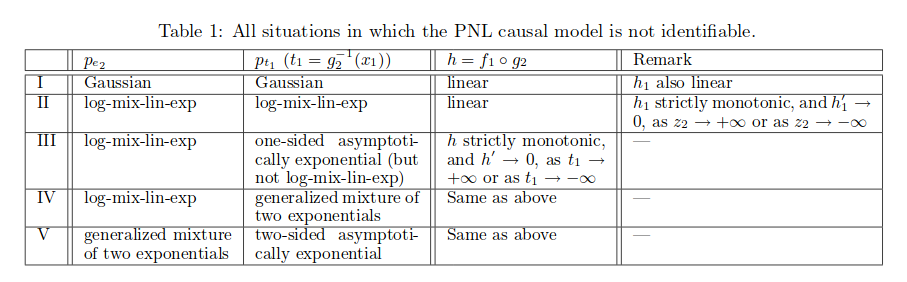
\includegraphics[scale=0.5]{pnl.png}
\caption{تمام حالاتی که در آن مدل قابل شناسایی نیست.}
\label{PNL}
\end{figure}


\subsection{مقایسه‌ی نتایج}
در این بخش سه مقاله‌ی اصلی که قضایای 
\lr{identifiablity}
مربوط به مدل‌های نویز جمعی ارائه داده‌اند را بررسی کردیم. در ادامه به مقایسه این مقالات می‌پردازیم.


مقاله‌ی 
\lr{Hoyer et. al}
برای اولین بار مدل‌های نویز جمعی را معرفی می‌کند و قضیه‌ی 
\lr{identifiablity}
دو بعدی را ثابت می‌کند که سنگ‌بنای تمام کار‌های بعدی این حوزه است. این مقاله نتایج خود را با داده‌‌های واقعی و همچنین داده‌های مصنوعی نیز می‌سنجد. یک نقطه‌ی ضعف این مقاله این است که در آزمایش‌های تجربی خود، حالت‌هایی به جز حالت گاوسی-خطی که در آن \lr{identifiablity}
نداریم را بررسی نمی‌کند. این ایراد در تمام مقالات بعدی نیز وجود دارد.

مقاله‌ی 
\lr{Peters et al.}
با ارائه‌ی شیوه‌ای برای تعمیم قضایای 
\lr{identifiablity}
به چند بعد، قدم بزرگی در استنتاج‌علی بر می‌دارد که حتی در بیرون از مدل‌های نویز جمعی نیز کاربرد وسیع دارد. الگوریتم 
\lr{RESIT}
که در این مقاله معرفی ‌می‌شود نیز تا کنون جز بهترین ابزارهای یادگیری ساختار علّی باقی‌مانده است و ایده‌ی آن در مقالاتی مثل 
\cite{time}
نیز به کار رفته است. بخش آزمایش‌ الگوریتم بر روی داده‌های واقعی این مقاله ضعف‌های اساسی دارد. این مقاله الگوریتم خود را تنها بر روی یک دیتاست می‌آزماید که در این دیتاست، جهت درست علّی به درستی مشخص نیست. در ادامه بیشتر به الگوریتم 
\lr{RESIT}
خواهیم پرداخت.

مقاله‌ی 
\lr{Zhang}
قضیه  
\lr{identifiablity}
بسیار قوی‌ای برای مدل‌های 
\lr{Post Non-Linear}
ارائه داده است که می‌توان با روش مقاله‌ی 
\cite{continous}
به راحتی آن را به حالت چند متغیره نیز تعمیم داد. برای یادگیری
\lr{Post Non-Linear}
ها، تاکنون الگوریتم یادگیری مناسبی ارائه نشده است. به نظر من 
\lr{Post Non-Linear}
ها هنوز به بلوغ کامل نرسیده‌اند و باید کار بسیار بیشتری بر روی الگوریتم‌های یادگیری آن‌ها انجام شود.
\section{الگوریتم‌های یادگیری}

در این بخش به بررسی الگوریتم‌های یادگیری گراف مربوط به یک 
\lr{SCM}
از داده‌ی محدود به فرض اینکه  در
\lr{SCM}
مدل نویز جمعی برقرار باشد، پرداخته و الگوریتم‌های مختلف مطرح شده را با هم مقایسه می‌کنیم. مراجع ما در این بخش مقالات 
\cite{continous}
و 
\cite{nowzohour}
هستند.
\subsection{الگوریتم 
	\lr{RESIT}
}
این الگوریتم توسط 
\lr{Peters et al.}،
سال ۲۰۱۴، در
\cite{continous}
معرفی شده است. ایده‌ی اصلی این الگوریتم این است که برای هر $X_i$ اگر $X_i$ یک
\lr{Sink Node}
باشد داریم
$N_i \bigCI \mathbf{X} \setminus \{X_i\}$
به طور کلی برای هر 
$Y \in \mathbf{X}$،
$N_Y \bigCI \mathbf{ND}_Y$.

\begin{latin}	
	\begin{algorithm}[h]
		\caption{Regression with subsequent independence test (RESIT)}
		\label{alg:icml}
		\begin{algorithmic}[1]
			\STATE {\bfseries Input:} i.i.d. samples of a $p$-dimensional distribution on $(X_1, \ldots, X_p)$ \vspace{0.0cm}
			\STATE $S:=\{1, \ldots, p\}, \pi := [\ ]$ \vspace{0.15cm}
			\STATE PHASE 1: Determine causal order.
			\REPEAT
			\FOR{$k \in S$}
			\STATE Regress $X_k$ on $\{X_i\}_{i \in S \setminus \{k\}}$.% (and $X^i_t$ for instantaneous effects).
			\STATE Measure dependence between residuals and $\{X_i\}_{i \in S \setminus \{k\}}$.  
			\ENDFOR
			\STATE Let $k^*$ be the $k$ with the weakest dependence.
			\STATE $S:=S \setminus \{k^*\}$
			\STATE $\mathrm{pa}(k^*):=S$
			\STATE $\pi := [k^*, \pi]\qquad $  ($\pi$ will be the causal order, its last component being a sink)
			\UNTIL{$\#S=1$} \vspace{0.15cm}
			\STATE PHASE 2: Remove superfluous edges.
			\FOR{$k \in \{2, \ldots, p\}$}
			\FOR{$\ell \in \mathrm{pa}(\pi(k))$}
			% \STATE Remove all superfluous parents from $\mathrm{pa}(k)$ that are not required to obtain independent residuals
			\STATE Regress $X_{\pi(k)}$ on $\{X_i\}_{i \in \mathrm{pa}(\pi(k)) \setminus \{\ell\}}$.
			\IF{residuals are independent of $\{X_i\}_{i \in \{\pi(1), \ldots, \pi(k-1)\}}$} % (i.e., of the variables appearing earlier in the causal order)
			\STATE $\mathrm{pa}(\pi(k)) := \mathrm{pa}(\pi(k)) \setminus \{\ell \}$ 
			\ENDIF
			\ENDFOR
			\ENDFOR
			%   \STATE Check the remaining indep. to verify the model.
			%   \IF{model correct}
			\STATE {\bfseries Output:} $(\mathrm{pa}(1), \ldots, \mathrm{pa}(p))$
			%   \ELSE
			%   \STATE {\bfseries Output:} I do not know - bad model fit.
			%   \ENDIF
		\end{algorithmic}
	\end{algorithm}
\end{latin}	
الگوریتم 
\lr{RESIT}
در هر مرحله یک 
\lr{Sink Node}
را تشخیص داده و حذف می‌کند. برای تشخیص یک 
\lr{Sink}
نیز از ويژگی $N_i \bigCI \mathbf{X} \setminus \{X_i\}$ استفاده می‌کند. 


الگوریتم 
\lr{RESIT}
دو فاز دارد. در فاز اول (خط ۳ تا ۱۳)، یک 	\lr{Causal Order} پیدا می‌شود. با رگرس کردن هر متغیر روی بقیه‌ی متغیر‌های گراف هر مرحله، متغیری که باقی مانده‌ی رگرسیون مربوط به از دیگر متغیرها مستقل‌تر(مثلاً با معیار 
\lr{p-value}
آزمون 
\lr{HSIC}) باشد را به عنوان یک  
\lr{sink}
در نظر می‌گیریم. با حذف این راس، مجدداً یک
\lr{DAG}
دیگر به وجود می‌آید که در آن همین روند را روی آن تکرار می‌کنیم. با این کار می‌توان به یک 
\lr{Causal Order}
برای متغیرها رسید.
در فاز دوم، برای شروع  فرض می‌شود که اگر
$\pi(i) < \pi(j)$،
از $i$ به $j$ یک یال وجود دارد . از این گراف شروع کرده. هر بار یک متغیر،
$X_{\pi(k)}$،
را در نظر گرفته و آن را بر روی 
\lr{parent}
هایش به جز یک 
\lr{parent}،
$X_l$،
رگرس می‌کنیم به نحوی که هر 
\lr{parent}
یک بار از رگرسیون کنار گذاشته شود. در هر رگرسیون، اگر باقی‌مانده رگرسیون از متغیر‌هایی که در 
\lr{Causal Order}
بالاتر از 
$X_{\pi(k)}$
هستند مستقل شد، ارتباط $X_l$ و $X_{\pi(k)}$ را حذف می‌کنیم. 

الگوریتم 
\lr{RESIT}
در مرحله‌ی اول خود 
$O(n^2)$
تست آماری انجام می‌دهد و در مرحله‌ی دوم نیز تعداد تست های آماری
$O(n)$
است. چند جمله‌ای بودن این الگوریتم بسیار عجیب است زیرا مسائل معمول در 
\lr{Bayesian Network Learning}
اکثراً 
\lr{NP-Hard}
هستند. با این وجود الگوریتم 
\lr{RESIT}
برای \lr{n} های بزرگ قابل استفاده نیست زیرا در صورتی که در انجام تست آماری دچار خطا شویم، خطا به شدت در مراحل بعد منتشر شده و باعث می‌شود به طور قابل ملاحظه‌ای از گراف اصلی دور شویم. 
\subsection{روش
	\lr{Brute Force}
	و 
	\lr{GDS}
}
یک دسته‌ی دیگر از الگوریتم‌های یادگیری در مدل‌های نویز جمعی، الگوریتم‌های مبتنی بر 
\lr{score}
هستند. 

برای یادگیری ساختار مدل‌های نویز جمعی محدود شده، ‌می‌توان تمام
\lr{DAG}
ها را 
\lr{enumerate}
کرد و بررسی کرد که آیا  استقلال‌هایی که از داده‌ها استخراج می‌شوند در گراف نیز وجود دارند  یا خیر. یک ایراد این روش  این است که این روش لزوما یک گراف
\lr{Causal Minimal}
به ما نمی‌دهد. برای حل این مشکل یک 
\lr{penalized independence score}
تعریف کرده و آن را برای گراف‌ها محاسبه می‌کنیم و این معیار را مبنای انتخاب گراف قرار می‌دهیم.
$$\hat{G} = \mathrm{argmin}_G \sum_{i=1}^n \mathrm{DM}(res_i^{G, \mathrm{RM}}, res_{-i}^{G, \mathrm{RM}}) + \lambda \#\mathrm{edges}$$
در آن 
\lr{RM}
روش رگرسیون ما و 
\lr{DM}
یک معیار استقلال است.
$res_i$
مقدار باقی مانده‌ی رگرسیون $X_i$ است وقتی آن را بر روی تمام 
\lr{parent}
هایش رگرس می‌کنیم و 
$res_{-i}$
باقی‌مانده‌ی رگرسیون مابقی متغیر ها به جز $X_i$ است. واضح است که این الگوریتم برای گراف‌های بزرگ به هیچ وجه قابل استفاده نخواهد بود.

یک راه معقول برای کاهش پیچیدگی محاسباتی الگوریتم فوق، استفاده از روش‌های حریصانه است
\cite{continous}.
دو گراف را مجاور می‌گوییم اگر تنها با یک تغییر جهت، افزودن یال یا کاستن یال به یکدیگر تبدیل شوند. در الگوریتم حریصانه، در هر مرحله 
\lr{score}
گراف آن مرحله را حساب کرده و با 
\lr{score}
گراف‌های مجاور مقایسه‌ می‌شود. هرجا امتیاز یکی از این گراف‌های مجاور از گراف اصلی بالاتر بود، گراف اصلی را برابر گراف مجاور می‌گذاریم و الگوریتم را ادامه می‌دهیم. برای اینکه استپ‌ها کمی بهتر شوند، به صورت تصادفی امتیاز همسایه‌ها را محاسبه نمی‌کنیم بلکه از همسایه‌ای شروع می‌کنیم که باقی‌مانده آن نسبت به باقی ‌مانده‌ی دیگر راس‌ها کمتر مستقل است. تضمینی وجود ندارد که این روش به بهترین گراف برسد
\cite{continous}.
نویسندگان مقاله حتی ادعای مبنی بر این موضوع نیز انجام نمی‌دهند.

\subsection{مقایسه‌ی الگوریتم‌های‌
\lr{RESIT}،
\lr{Brute Force} و 
\lr{GDS}
با سایر الگوریتم‌ها
}
مقاله‌ی 
\cite{continous}
به صورت مفصل الگوریتم‌های \lr{RESIT}،
\lr{Brute Force}, 
\lr{GDS}، \lr{GES}
\lr{PC},
و
\lr{LiNGAM}
را مقایسه می‌کند. در ادامه به بررسی این مقایسه و نقد آن می‌پردازیم. 
\textbf{ایراد بزرگ این مقایسه این است که بر روی داده‌هایی انجام شده که به صورت مصنوعی تولید شده‌اند.}
معیار مورد استفاده‌ی ما برای مقایسه‌ی الگوریتم‌ها  \textbf{\lr{Structural Hamming Distance (SHD)}} است.
	همان‌طور که از اسم این معیار بر می‌آید، این معیار تعداد یال‌های اشتباه را می‌شمارد. وجود هر یال اضافه یا جهت‌دار به دست‌آوردن یال بی‌جهت نیز یک خطا در نظر گرفته می‌شود. در جدول‌های مقایسه‌ای که در بخش‌های بعد خواهند آمد، ردیف 
	\lr{DAG}
	مقایسه‌ی 
	\lr{DAG}
	واقعی با گراف به دست آمده  و ردیف
	\lr{CDAG}
	مقایسه‌ی
	\lr{CDAG}
	و گراف حاصل است.  
	

\subsubsection{
حالت
\lr{SCM}
خطی
}
در حالت خطی، ضرایب 
 $\beta_{jk}$
 به صورت تصادفی با توزیع یکنواخت 
 $[-2,-0.1] \cup [0.1,2]$
 انتخاب می‌شوند. نویز های برونی مستقل هستند و با توزیع 
 $K_j \cdot \mathrm{sign}(M_j)\cdot |M_j|^{\alpha_j}$
 تولید می‌شوند که در آن
 $M_j \stackrel{}{\sim} N(0,1)$, $K_j \stackrel{}{\sim} U([0.1,0.5])$ 
 و
  $\alpha_j \stackrel{}{\sim} U([2,4])$. 
\begin{figure}[h!]
	\centering
	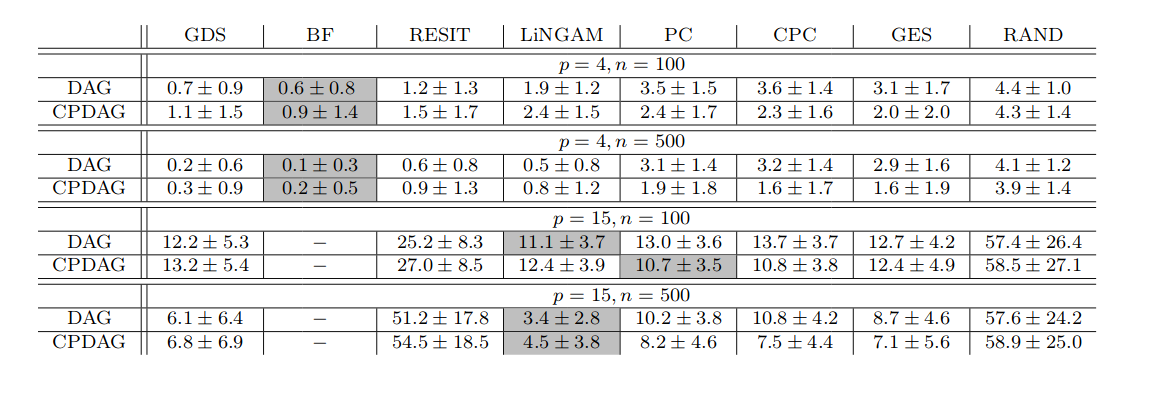
\includegraphics[scale=0.42]{linear.png}
	\caption{SHD
الگوریتم‌های مختلف به ازای گراف‌هایی با سایز‌های مختلف	 - مدل خطی
}
\label{linearSCM}
\end{figure}
جدول  \eqref{linearSCM} مقایسه‌ی 
\lr{SHD}
این الگوریتم‌ها برای گراف‌ها با تعداد راس مختلف است. 
در این جدول، روش 
\lr{RAND}
به این نحو است که به صورت کاملاً تصادفی یک گراف انتخاب کرده و به داده‌ها نسبت می‌دهیم. 
\begin{itemize}
\item 
همان‌طور که انتظار می‌رفت، در گراف‌های کوچک، بررسی تمام گراف‌ها بهترین نتیجه را داشته ولی برای گراف‌های بزرگ، امکان اجرای این الگوریتم نبوده است.
\item 
در گراف‌های بزرگ‌تر روش 
\lr{LiNGAM}
بهترین نتیجه را دارد. نکته‌ی جالب این است که روش 
\lr{DAG}
نیز حاصلی شبیه به روش 
\lr{LiNGAM}
دارد که نشان می‌دهد روش 
\lr{GAS}
 در کمینه‌های موضعی گیر نیفتاده است.
 \item 
 مطابق انتظار، الگوریتم
 \lr{REST}
 در حالت خطی بسیار ناموفق عمل کرده است. این عدم موفقیت، به خصوص در گراف‌هایی با تعداد رأس زیاد بسیار شدید است. دلیل این امر این است که این الگوریتم، در این حالت در فاز اول خود یال‌های اضافی زیادی نگه می‌دارد که در فاز دوم قابل حذف نیستند.

\end{itemize}

\subsubsection{حالت 
\lr{SCM}
غیرخطی
}
در این حالت، تابع به صورت تصادفی از  یک فرآیند گاوسی با پهنای باند ۱ انتخاب شده و نویز‌ها گاوسی هستند و واریانس آن تصادفی انتخاب شده است.
در حالت غیرخطی نیز مشابه حالت خطی، در گراف‌های کوچک روش 
\lr{Brute Force}
بهترین نتیجه را می‌دهد. روش 
\lr{GDS}
نیز مشابه روش 
\lr{Brute Force}
عمل می‌کند. با بزرگتر شدن سایز گراف، دیگر روش 
\lr{Brute Force}
قابل استفاده نیست و روش
\lr{GDS}
هم کارایی خود را از دست داده و گرفتار کمینه‌های موضعی می‌شود. به نظر می‌رسد که در گراف‌های بزرگتر الگوریتم
\lr{RESIT}
موفق‌تر از سایر روش‌ها عمل می‌کند. بهتر بود که این مقاله برای گراف‌های بزرگتر نیز این الگوریتم‌ها را تست می‌کرد تا بتوانیم با اطمینان بیشتری گزاره‌ی بهتر بودن روش 
\lr{RESIT}
از سایر روش‌ها در گراف‌های بزرگ‌تر را مطرح کنیم.

\begin{figure}[h!]
\centering
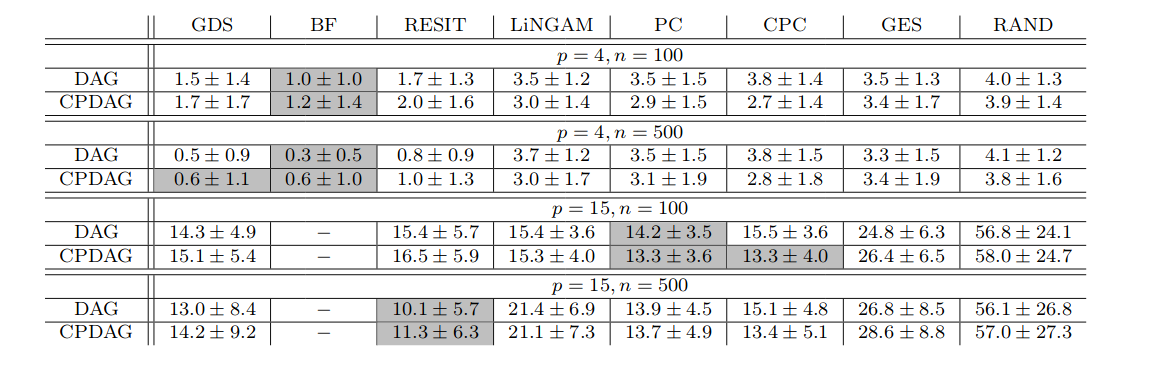
\includegraphics[scale=0.42]{dif.png}
	\caption{SHD
	الگوریتم‌های مختلف به ازای گراف‌هایی با سایز‌های مختلف	 - مدل غیرخطی
}
\end{figure}

\subsubsection{بررسی داده‌های واقعی؟!}
در ادامه این مقاله تلاشی مذبوحانه(!) برای اثبات کارآمدی الگوریتم 
\lr{RESIT}
انجام می‌دهد.

داده‌ی مورد استفاده، سه متغیر‌ مشاهده شده دارد: دمای شهر، ارتفاع شهر و مدت زمان تابش خورشید. این داده از ۳۴۹ مرکز هواشناسی آلمان به دست آمده است.
\begin{figure}[h!]
	\begin{center}
		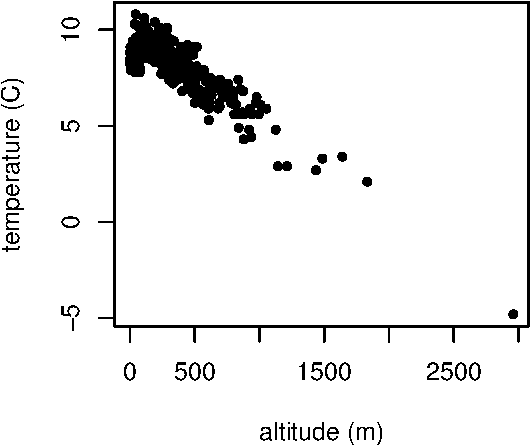
\includegraphics[width=0.31\textwidth]{experimentAltTempcut}
		\hspace{0.02\textwidth}
		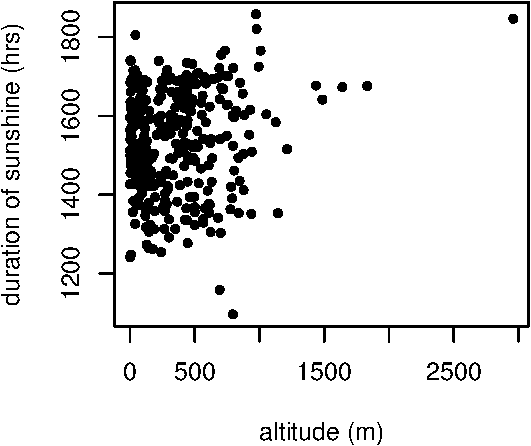
\includegraphics[width=0.31\textwidth]{experimentAltSuncut}
		\hspace{0.02\textwidth}
		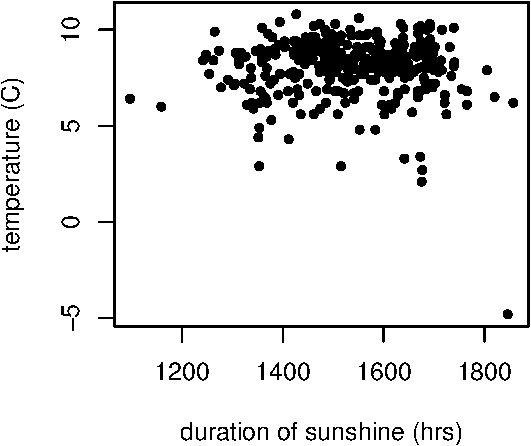
\includegraphics[width=0.31\textwidth]{experimentSunTempcut}
	\end{center}
	\caption{نمودار پراکنش داده‌های مسئله}
	\label{fig:alt}
\end{figure}

\begin{center}

\begin{figure}
\centering
\begin{latin}
\begin{tabular}{| c| c |}
\hline
Method & Graph \\
\hline\hline
LiNGAM & $T \rightarrow A$ \\
\hline
PC &  $T \rightarrow A \leftarrow DS$ \\
\hline
CPC& $T \rightarrow A \leftarrow DS$ \\
\hline
GES& Fully Connected\\
\hline
GDS& $T \leftarrow A \rightarrow DS$\\
\hline
BF& $T \leftarrow A \rightarrow DS$\\
\hline
RESIT&$T \leftarrow A \rightarrow DS$\\
\hline
\end{tabular}
\end{latin}
\caption{گراف پیشنهادی الگوریتم‌های مختلف}
\end{figure}

\end{center}
دیده می‌شود که الگوریتم‌های 
\lr{LiNGAM}،
\lr{(C)PC}،
\lr{GES}
گراف‌هایی را پیشنهاد می‌کنند که به وضوح غلطند! زیرا 
\lr{Intervention}
برو روی دمای شهر و یا زمان تابش خورشید در یک شهر، تاثیری بر روی ارتفاع آن نخواهد داشت. سه روش 
\lr{GES}،
\lr{BF} 
و
\lr{RESIT}
جواب‌های مشابهی می‌دهند. 

به نظر من این گراف‌ها غلط هستند زیرا علاوه بر دو یالی که \lr{RESIT}
می‌یابد،  چنین یالی نیز در گراف موجود باشد: $T \leftarrow DS$. نویسنده‌ی مقاله بیان می‌کند که گرافی که هر سه یال را دارد، در الگوریتم های 
\lr{GES}
و
\lr{BF} 
دومین بالاترین 
\lr{score}
را می‌یابد و ادعا می‌کند که این اشتباه به دلیل وجود 
\lr{confounder}
هایی از جنس متغیر‌های جغرافیایی است. 

به نظر من این تحلیل به هیچ عنوان تحلیل جامع و دقیقی برای مقایسه‌ی الگوریتم‌ها نیست. اولاً این مطالعه تنها بر روی یک دیتاست انجام شده است، حتی برای بدترین لگوریتم‌ها نیز می‌توان یک دیتاست یافت که خروجی آن الگوریتم جواب مناسبی باشد. دوماً جواب این الگوریتم خیلی جواب خوبی نیز نیست! سوماً اینکه 
\textbf{
تعداد متغیر‌های این دیتاست بسیار محدود است و برای آزمودن الگوریتمی که ادعای چندمتغیره بودن دارد و با پشتوانه‌ی داده‌های مصنوعی، در مورد آن این ادعا شده است که در گراف‌هایی با تعداد متغیر بالا از الگوریتم‌های گذشته بهتر عمل می‌کند، کافی نیست.}

\section{متغیر‌های پنهان}
تا کنون کار زیادی بر روی یافت متغیر‌های پنهان در مدل‌های نویز جمعی انجام نشده است. یکی از معدود مقالات این حوزه، مقاله‌ی 
\cite{confounder}
است. در این مقاله، الگوریتمی به نام 
\lr{ICAN}
معرفی می‌شود که در حالت دو بعدی، می‌تواند وجود یک متغیر پنهان را تشخیص دهد.

\subsection{روش ساده‌لوحانه}
در وهله‌ی برای یافتن متغیر‌ پنهان، روش زیر به ذهن می رسد.

 فرض کنید 
	\begin{equation*}
	\begin{cases}
	X = f(T) + N_X\\
	Y = g(T) + N_Y
	\end{cases}
	\end{equation*}
می‌توانیم به روشی مشابه روش‌های
\lr{Dimension Reduction}
عمل کنیم. فرض کنید $(X_k, Y_k)$ داده‌هایی باشند که در اختیار ما هستند. برای یک خم دلخواه 
$\mathbf{s}(t)$
تعریف کنید
$$\hat{T}_k = \mathrm{argmin}_{t\in[0,1]} ||(X_k, Y_k) - \mathbf{s}(t)||_2$$ 
قصد داریم 
$\hat{\mathbf{s}}$ 
را بیابیم که
$\sum^n_{k=1} ||(X_k, Y_k) - \mathbf{s}(\hat{T}_k)||_2$. 
بعد از یافتن این خم، بررسی کنیم که آیا $(\hat{T}_k)$
و
$$(N_x, N_y) = (X, Y) - \mathbf{s}(\hat{T})$$
مستقل هستند یا خیر. این روش با وجود معقول بودن، در بسیاری از موارد ساده نیز بسیار بد عمل می‌کند.
\subsection{الگوریتم \lr{ICAN}}
برای رفع مشکلات الگوریتم ساده‌لوحانه، الگوریتم
\lr{ICAN}
ارائه شده است. در این الگوریتم از خم فوق به عنوان یک نقطه‌ی شروع استفاده می‌کند ولی به دنبالی خمی می‌گردد که نویز‌ها تا حد امکان از همدیگر مستقل شوند. 

\begin{figure}[h!]
	\begin{center}
		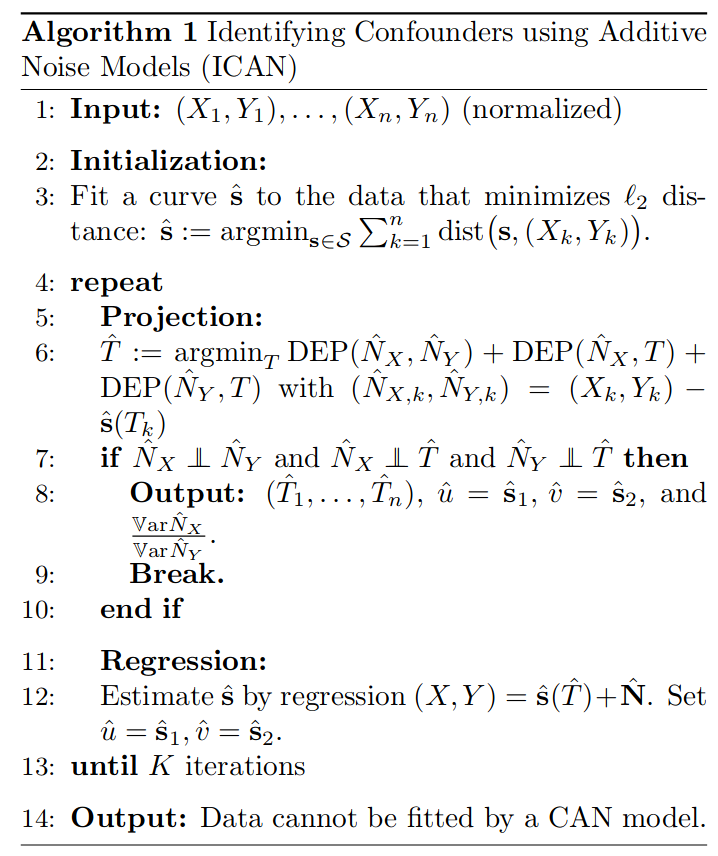
\includegraphics[width=0.5\textwidth]{ican.png}
	\end{center}
\end{figure}
اگر جهت علّی از $X$ به $Y$ باشد، به راحتی دیده ‌می‌شود که خمی که این الگوریتم باز می‌گرداند منجر به این نتیجه می‌شود که 
$\mathbf{var}\{\hat{N}_x\}<<\mathbf{var}\{\hat{N}_y\}$
از این ویژگی برای این استفاده خواهیم کرد که وجود یک متغیر پنهان را تشخیص دهیم.  شبه کد این الگوریتم در صفحه‌‌ی بعد آورده شده است.

مقاله اثباتی برای قابل‌شناسایی بودن،
\lr{identifiability}
برای  این الگوریتم ارائه می‌کند. نکته‌ی اصلی این مقاله این است که این قضیه تنها برای رژیمی که در آن واریانس نویز بسیار کم است ارائه شده و اثبات آن به شدت بر این فرض استوار است. داده‌های تجربی نشان می دهد که این روش می‌تواند در حالتی که واریانس نویز بزرگ است نیز موفق عمل کند، در نتیجه به نظر می‌رسد که قید کوچک بودن واریانس، تنها به دلیل ضعف اثبات است و انتظار می‌رود بتوان قضیه‌ی 
\lr{identifiability}
کلی‌ای، مشابه قضیه‌ی ارائه شده در
\cite{hoyer}
برای آن ارائه داد. این تلاش تا کنون ناموفق باقی مانده ‌است. از آن‌جا که اثبات تا حدی طولانی است، از آوردن  آن خودداری کردیم.


\subsection{بررسی تجربی الگوریتم}
\subsubsection{داده‌ی مصنوعی}
یک بررسی الگوریتم که در مقاله مطرح شده، به این شیوه بوده است:
 مدل
\begin{equation*}
\begin{cases}
X = f(T) + N_X\\
Y = g(T) + N_Y
\end{cases}
\end{equation*}
را در نظر گرفته و توابع $u$  و  $v$ را به صورت  تصادفی به صورت ترکیب خطی از توابع گاوسی انتخاب می‌کند و ۲۰۰ نقطه با کمکم آن تولید می‌کند. توزیع نویز
$U[−0.035,0.035]$
است. آزمون فرضیه‌ی استقلال مورد استفاده، آزمون 
\lr{HSIC}
است. نتیجه‌ی این آزمایش به شدت امیدوارکننده است. دیده‌ می‌شود که الگوریتم به درستی قادر به تشخیص مقدار 
\lr{confounder}
است و تنها آن را در 
$-1$
ضرب کرده، یک پارامتری‌کردن دیگر خم. شکل
\eqref{ican1}
بررسی نتایج این الگوریتم بر داده‌ی یادشده است.
\begin{figure}[h!]
	\begin{center}
		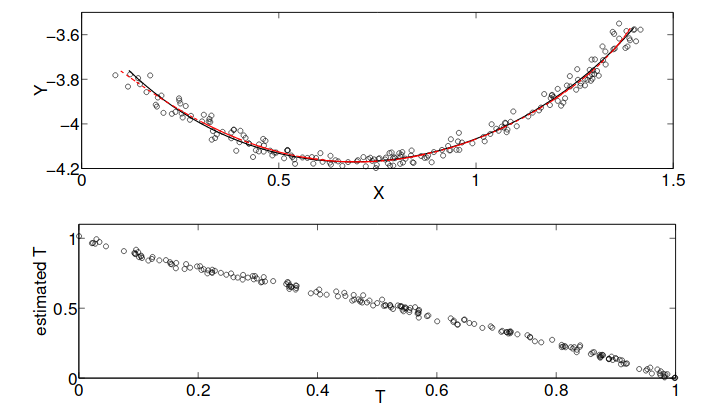
\includegraphics[width=0.5\textwidth]{ican1.png}
	\end{center}
	\caption{
		بررسی مقدار متغیر پنهان در داده‌های مصنوعی که توسط الگوریتم تشخیص داده شده است و مقایسه‌ی آن با مقدار واقعی.
	}
\label{ican1}
\end{figure}

\subsubsection{داده‌ی واقعی}
برای بررسی الگوریتم روی داده‌‌های واقعی، از داده‌ی معروف
\lr{The
	Automated
	Surface
	Observations
	Systems
	(ASOS) }
استفاده شده است. این دیتاست‌ متشکل از داده‌های ارسالی چند ایستگاه است که هر دقیقه داده‌های آب و هوا را مخابره می‌کنند. از داده‌های فشار هوا که از ایستگاه‌های 
\lr{KABE}
و
\lr{KABI}
در سال ۲۰۰۰ گرفته شده استفاده شده است. انتظار بر این است زمان یک 
\lr{confounder}
برای آن‌ها باشد. الگوریتم نیز یک 
\lr{confounder}
تشخیص می‌دهد و نتایج آن به طور کامل با این فرض هم‌‌خوانی دارند. 

\begin{figure}[h!]
	\begin{center}
		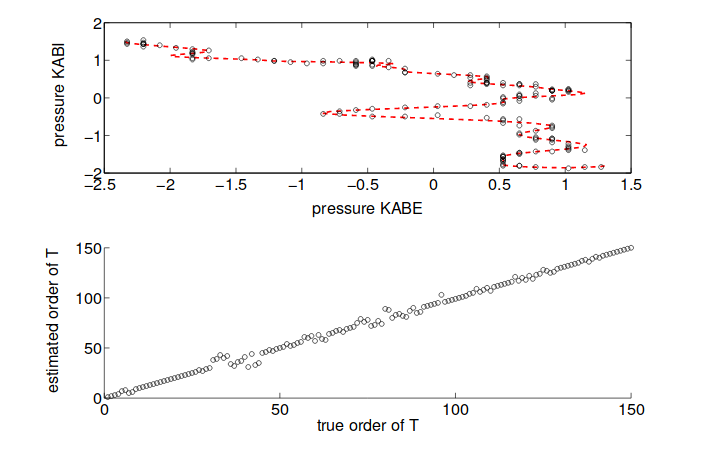
\includegraphics[width=0.5\textwidth]{kabe.png}
		\caption{
			بررسی مقدار متغیر پنهان در دیتاست واقعی که توسط الگوریتم تشخیص داده شده است و مقایسه‌ی آن با مقدار واقعی. 
		}
	\end{center}
\end{figure}

\section{سری‌های زمانی}
یکی از مدل‌های موفق و مبتنی بر محدود کردن مجموعه‌ی توابع، در سری‌های زمانی، الگوریتم‌های 
\lr{TiMINo}
است.
\begin{den} \label{def:timino}
	یک سری زمانی در نظر بگیرید.
	$X_t=(X^i_t)_{i \in V}$،
	به نحوی که توزیع‌های متناهی‌بعد آن تابع چگالی احتمال دارند. می‌گویم این سری زمانی یک 
	\lr{TiMINo}
	است اگر وجود داشته باشد
$p>0$ 
و 
$\forall i \in V$ 
مجموعه‌هایی وجود دارد که
 $\textbf{PA}ـ{i}^{0} \subseteq X^{V\setminus\{i\}}, \textbf{PA}_{i}^{k} \subseteq X^V$، 
 به نحوی که 
  $\forall t$
	\begin{align} \label{anm}
	X^i_t = f_{i}\big((\textbf{PA}_i^p)_{t-p}, \ldots, (\textbf{PA}_i^1)_{t-1}, (\textbf{PA}_{i}^{0})_{t}, \eps^i_t\big)\,,
	\end{align}
که در آن 
$\eps^i_t$ 
(مشترکاً) مستقل هستند و برای هر $i$،
$\eps^i_t$ 
در زمان 
\lr{identically distributed}
است. همچنین فرض بر این است که 
\lr{Full Time Graph}
دور ندارد.
\end{den}

این مدل می‌تواند به راحتی به یک مدل نویز جمع شونده تبدیل شود. می‌توان با اندکی تلاش، از قضیه‌ی اثبات شده در 
\cite{hoyer}
برای دو متغیر و تعمیم آن در 
\cite{continous}
به یک قضیه‌ی 
\lr{identifiability}
برای سری‌های زمانی 
\lr{TiMINo}
با فرض نویز جمعی رسید.


مقاله‌ی 
\cite{time}
الگوریتمی ساده برای یافتن جهت‌های علّی در 
\lr{TiMINo}
ارائه می‌کند. این الگوریتم شباهت زیادی به الگوریتم  
\lr{RESIT}
دارد.
\begin{latin}
\begin{algorithm}[h!]
	\caption{TiMINo causality}
	\begin{algorithmic}[1]
		\STATE {\bfseries Input:} Samples from a $d$-dimensional time series of length $T$: $(\X_1, \ldots, \X_T)$, maximal order $p$\vspace{0.0cm}
		\STATE $S:=(1, \ldots, d)$ 
		\REPEAT
		\FOR{$k$ in S}
		\STATE Fit TiMINo for $X^k_t$ using $X^k_{t-p}, \ldots,$ $X^k_{t-1}, X^i_{t-p}, \ldots, X^i_{t-1}, X^i_t$ for $i \in S \setminus \{k\}$% (and $X^i_t$ for instantaneous effects).
		\STATE Test if residuals are indep. of $X^i, i \in S$.  
		\ENDFOR
		\STATE Choose $k^*$ to be the $k$ with the weakest dependence. (If there is no $k$ with independence, break and output: ``I do not know - bad model fit'').
		\STATE $S:=S \setminus \{k^*\}$
		\STATE $\mathrm{pa}(k^*):=S$
		\UNTIL{length(S)=1}
		\STATE For all $k$ remove all unnecessary parents.\vspace{0.0cm}
		%   \STATE Check the remaining indep. to verify the model.
		%   \IF{model correct}
		\STATE {\bfseries Output:} $(\mathrm{pa(1)}, \ldots, \mathrm{pa(d)})$
		%   \ELSE
		%   \STATE {\bfseries Output:} I do not know - bad model fit.
		%   \ENDIF
	\end{algorithmic}
\end{algorithm}
\end{latin}
ایده‌ی این الگوریتم استفاده از یک روش رگرسیون برای 
\lr{fit}
کردن یک 
\lr{TiMINo}
بر داده‌ها است با این فرض که می‌خواهیم کمترین تعداد والد ممکن برای رسیدن به نویز مستقل را داشته باشیم. برای استفاده از این الگوریتم باید یک روش رگرسیون را مشخص کنیم. به طور خاص در این مقاله از روش‌های 
\lr{gam}
و
\lr{GP}
استفاده شده است.

\subsection{
	مزایای \lr{TiMINo} بر سایر روش‌ها
}
\lr{TiMINo}
مزیت‌هایی بر سایر روش‌های تشخیص جهت علّی در سری‌های زمانی، به خصوص 
\lr{Granger Causality}
دارد که برخی از آنها را در ادامه خواهیم دید و مثال‌هایی از عملکرد روش ‌های مختلف خواهیم زد.
\begin{itemize}
	\item 
	\lr{TiMINo}
به وجود متغیر های مخفی نسبت به 
\lr{Granger Causality}
مقاوم‌تر است. علّت این مقاومت این است که در صورتی که موفق به مستقل کردن نویز‌ها نشود، بیان می کند که قادر به تشخیص جهت علّی نیست. به عنوان مثال به مثال زیر توجه کنید. در این گراف، $z$ یک متغیر پنهان است.
\begin{figure}[h!]
	\begin{center}
		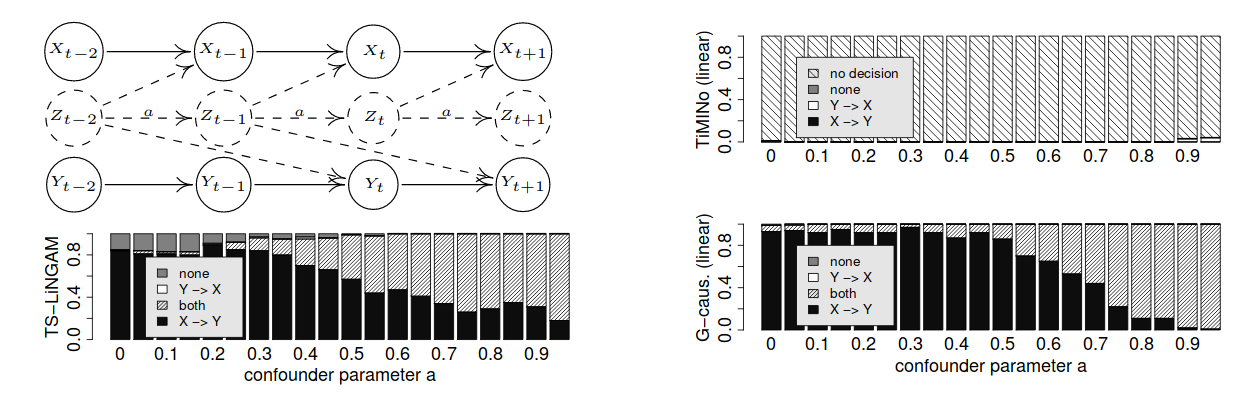
\includegraphics[width=\textwidth]{confounder.png}
		\caption{
تاثیر متغیر‌های پنهان در عملکرد الگوریتم‌های مختلف
		}
	\end{center}
\end{figure}
در این مثال با تغییر پارامتر‌ $a$ در گراف مشخص شده، نشان داده شده است که الگوریتم‌های مختلف در چه کسری از مواقع، 
\lr{summary graph}
اشتباهی را بازگرداند. مشاهده می‌شود با افزایش $a$، 
\lr{Granger Causality}
و 
\lr{TS-LiNGAM}
هر دو جهت را به عنوان جهت درست علّی معرفی می‌کنند ولی 
\lr{TiMINo}
همواره بیان ‌می‌کند که جهت قابل شناسایی نبود.
\item 
\lr{TiMINo}
نیازی به فرض عدم وجود 
\lr{instantaneous effect}
ندارد. 
 
 به عنوان مثال  سری‌های زمانی زیر را در نظر بگیرید.
$X_t=A_1\cdot X_{t-1}+\eps_{X,t},
W_t=A_2\cdot W_{t-1}+A_3\cdot X_{t}+\eps_{W,t},
Y_t=A_4\cdot Y_{t-1}+A_5\cdot W_{t-1}+\eps_{Y,t},
Z_t=A_6\cdot Z_{t-1}+A_7\cdot W_t+A_8\cdot Y_{t-1}+\eps_{Z,t}
$

$\eps_{\cdot, t} \sim 0.4 \cdot \mathcal N(0,1)$ 
و
 $A_i$ 
 از توزیع
$\mathcal{U}([-0.8,-0.2]\cup [0.2,0.8])$
آمده است.
در این بررسی، گراف
 $X \rightarrow W \rightarrow Y \rightarrow Z$ و  $W \rightarrow Z$ 
 را به عنوان گراف صحیح در نظر گرفته‌ایم. موفقیت الگوریتم‌های مختلف برای تشخیص جهت علّی بدین صورت است.
 
 \begin{figure}[h!]
 	\begin{center}
 		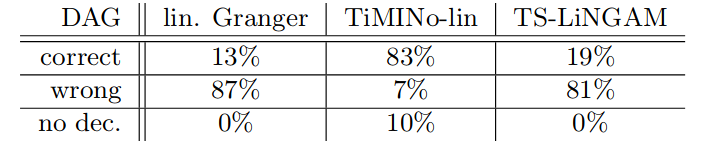
\includegraphics[width=0.65\textwidth]{ts.png}
 		\caption{
تاثیر اثرات آنی بر عملکرد الگوریتم‌های مختلف
 		}
 	\end{center}
 \end{figure}
مشاهده می‌شود که 
\lr{TiMINo}
مطابق انتظارات، توانسته از دو الگوریتم دیگر بسیار بهتر عمل کند.
\item 
ادعای بزرگ دیگری که در این مقاله مطرح شده اما به صورت تجربی آزمایش نشده این است که فرض کنید سیگنال‌ها از سورس‌های مختلف به ما می‌رسند و در نتیجه تاخیر‌های زمانی متفاوتی در دریافت آن‌ها داریم. به دلیل این تاخیر‌ها که از وجود آنها اطلاع نداریم، ممکن است جهت علّی معکوس در زمان نیز داشته باشیم. ادعا شده است که حتی در این حالت نیز
\lr{TiMINo}
قادر به تشخیص 
\lr{summary graph}
است.
\end{itemize}

به طور کلی، مقاله‌ی 
\cite{time}،
بررسی تجربی بسیار دقیقی روی 
\lr{TiMINo}
انجام می‌دهد. این مقاله، در مثال‌های واقعی زیادی الگوریتم 
\lr{TiMINo}
را آزمایش می‌کند. از جمله‌ی این آزمایش‌ها می‌توان به بررسی قیمت روزانه‌ی پنیر و کره پرداخت. انتظار این است که این دو سری زمانی، یک 
\lr{confounder}
مثل قیمت شیر داشته باشند. \lr{TiMINo} در این حالت جهت علّی تشخیص نمی‌دهد ولی دو روش 
\lr{TS-LiNGAM}
و
\lr{Granger Causality}
به اشتباه جهت‌هایی علّی ارائه می‌کنند.

\section{پیشنهاد برای کار‌های پژوهشی آتی}
به نظر من، در اولین قدم باید تلاشی برای یافتن یک قضیه‌ی 
\lr{identifiability}
کامل و بدون فرض کوچک بودن نویزها، که در 
\cite{confounder}
انجام شده است، انجام شود. این کار می‌تواند سنگ‌بنای کار‌های بزرگتری، مانند تعمیم نتایج آن و الگوریتم 
\lr{ICAN}،
به بعد‌های بالاتر باشد. 



مقاله‌ی 
\cite{continous}
بررسی تجربی دقیقی بر الگوریتم 
\lr{RESIT}
انجام نداده است. بررسی دقیق عملکرد این الگوریتم و مشاهده‌ی 
\lr{pithole}
های آن می‌تواند شهود بسیار بهتری برای ارائه‌های الگوریتم‌های یادگیری ساختار علّی دیگر به ما بدهد.


الگوریتم 
\lr{TiMINo}
به دلیل توانایی هندل کردن تاخیر‌های زمانی در سیگنال‌هایی که قصد یافتن جهت‌های علّی آن‌را داریم، می‌تواند در بررسی‌های 
\lr{Fumctional Connectivity}
در مغز بسیار مفید باشد. به طور خاص در داده‌های 
\lr{fMRI}
مشکل وجود تاخیر‌های مختلف زمانی مشاهده شده است.

الگوریتم یادگیری مناسب و بهینه‌ای برای 
 \lr{Post Non Linear Models}
 وجود ندارد در حالی که به نظر می‌رسد این مدل‌ها تا حد زیادی مطابق اندازه‌گیری‌های ما از طبیعت باشند، زیرا تابع بیرونی می‌تواند اندازه‌گیری ما را مدل کند. به نظر من این مدل‌ها، پتانسیل این را دارند توصیف‌گر دقیق‌تری از طبیعت باشند. همچنین تعمیم این مدل به مدل
 \begin{equation*}
\begin{cases}
X = N_X\\
Y = f(g(X) + N_y) + N_*
\end{cases}
 \end{equation*}
 با فرض استقلال
$ N_x, N_y, N_*$
 که در آن $N_*$ مدل‌کننده نویز اضافه شده بر دیتای اندازه‌گیری شده است و ارائه‌ی یک قضیه‌ی
 \lr{identifiability}
 احتمالی  برای این مدل‌ها خالی از لطف نیست.
\bibliographystyle{acm-fa}
\bibliography{bib}
\end{document}

